\chapter{Tutorial}
In this chapter, you will learn the basic operation of a test board setup, communication with the test board and a single chip.

\section{Requirements}
To work yourself through this tutorial, you need
\begin{itemize}
    \item A DTB, connected to your computer via USB
    \item A adapter board for a single chip
    \item A single chip holder, equiped with a chip (does not require a sensor)
    \item The software \texttt{psi46test} installed
    \item An oscilloscope, fast enough to resolve 200\,MHz signals
    \item NIM cables of equal length (i.e.\, 6\,ns delay or similar)
\end{itemize}
\todo{Find conistent names for the adapter card and the single chip card and use it consistently.}

If you need help to set this up, please go to the \enquote{How To's}, chapter \ref{sec:howto}.

\note{Whenever you do any change to the testboard (i.e.~switch adapter cards, switch chips etc.), make sure that the chip is not powered. To do so, check that the red LED labeled \enquote{RUN} is dark. If not, issue the command \psicommand{poff} from within \texttt{psi46test}.}

\section{Hello world}
For this test, connect an adapter card to the DTB but do not insert a chip holder.

%A first test is to see if supply voltages are present. Invoke \texttt{psi46test} and issue the command

A basic test is to see if we can trigger on a signal and see something. For this we program the built-in pulse generator to send a sync signal and a token. The sync signal is not routed to the chip. It is only used as a marker of the pulse sequence so that the oscilloscope has a meaningful signal to trigger on. Make the following connections:
\begin{itemize}
    \item Connect the \enquote{D1} output of the DTB to the first channel of your scope
    \item Connect the \enquote{A1+} output of the DTB to the second channel of your scope
\end{itemize}
Let us set a basic sequence:

\bigskip

\begin{tabular}{lp{0.6\textwidth}}
    \toprule
Command & Brief description \\
    \midrule
\psicommand{d1 9}              & This selects pg\_sync as signal routed to D1\\
\psicommand{a1 0}              & Select the token in signal as analog signal routed to A1\\
\psicommand{pgset 0 b100001 0} & Program the pulse generator to send a sync and a token out \\
\psicommand{pgloop 1000}       & Start the pulse generator. Repeats the pulse sequence infinitely, start a new cycle every 1000 clock cycles\\
    \bottomrule
\end{tabular}

\bigskip

One clock cycle is 25\,ns long, i.e.~the frequency is 40\,MHz, which coincides with the LHC bunch frequency.

Set up your scope to trigger on the first channel and you should see something like what is shown in Fig.~\ref{fig:tut_scope1}.
\begin{figure}[h]
    \begin{center}
	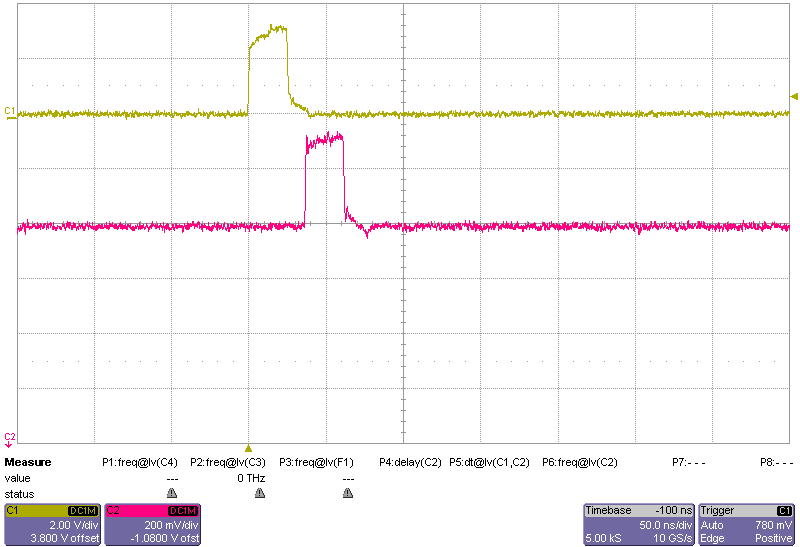
\includegraphics[width=0.7\textwidth]{img/tut_scope1.png}
	\caption{Output of first test. The first channel (yellow, top) shows the sync signal. It has a width of 25\,ns. The second signal is the token (red). It appears with some delay and has the same width.}
	\label{fig:tut_scope1}
    \end{center}
\end{figure}

Now let us see what this little sequence actually does. You can think of such a sequence as a little program. Using the command \psicommand{pgset} one can create pulse sequences to test different things. Our sequence has only one step where we create a pulse on the sync and the token signal. One step has a number, a bit pattern and a delay to the next pattern. If the delay is set to 0, the cycle ends, as it does in our example. The bit pattern is given as a binary number, starting with a \psicommand{p}. The following bits can be set:
\begin{center}
\begin{tabular}{lcccccc}
    \toprule
Bit:  & 0 & 1 & 2 & 3 & 4 & 5 \\
Name: & sync & reset TBM & reset ROC & calibrate & trigger & token \\
Abbreviated name: & (sync) & (rest) & (resr) & (cal) & (trg) & (tok) \\
    \bottomrule
\end{tabular}
\end{center}

Our example sends out a sync and a token signal, as we observed. So we understood what the sequence does. And we know that our setup works.

% px4.png

\psicommand{getid}


